\documentclass[12pt, a4paper]{article}
%IMPORTS
\usepackage{polski}
\usepackage[utf8]{inputenc}
\usepackage[a4paper, total={15cm, 24cm}]{geometry}
\usepackage[T1]{fontenc}

\usepackage{graphicx}
\usepackage[inkscapeformat=pdf]{svg}

\usepackage{url}
\usepackage{hyperref}
\hypersetup{
    colorlinks=true,
    linkcolor=blue,
    filecolor=magenta,      
    urlcolor=cyan,
    pdftitle={Overleaf Example},
}

\usepackage{amsmath}
\usepackage{bytefield}
\usepackage{siunitx}
\usepackage{minted}
\usepackage{circuitikz}
\usetikzlibrary{decorations.shapes}

\usepackage{biblatex}
\addbibresource{references.bib}

\graphicspath{{img/}}

\title{
	Generator sygnału \qty{1}{\kHz}\\
	\large Raport Techniczny
}

\author{Szymon Januszek, \texttt{szymon\_j@tutanota.com}}

\date{Kwiecień 2023}

\begin{document}
\normalfont
\fontfamily{lmtt}
\maketitle
\hrule

\begin{abstract}
	Głównym celem poniższej konstrukcji jest otrzymanie sygnału możliwie najwyższej jakości, 
	zdefiniowanych w założeniach konkursowych, tzn. dokładność częstotliwości, stopień zniekształceń harmonicznych 
	oraz dokładność amplitudy sygnału.
\end{abstract}

%TODO: fancy graphics

\newpage

\tableofcontents

\newpage

\section{Bezpośrednia synteza cyfrowa}

Aby wygenerować maksymalnie stabilny i dokładny względem częstotliwości sygnał, 
zdecydowałem się na wykorzystanie techniki \verb|Bezpośredniej Syntezy Cyfrowej|, 
gdzie mikroprocesor wraz z układem Przetwornika Cyfrowo-Analogowego (DAC) generuje sygnał zbliżony do sygnału oczekiwanego. 
Umożliwia to zastosowanie wysokiej jakości generatora kwarcowego, 
jako głównego źródła odniesienia, o precyzji rzędu 50ppm\footnote{Części na milion}, 
w całym zakresie temperatur. Oznacza to, iż częstotliwość uzyskanego sygnału nie będzie odbiegać o więcej niż $\pm$\qty{50}{\mHz} od wartości oczekiwanej. 

\subsection{Mikrokontroler}
Jako główny mikrokontroler wybrany został układ \textbf{AVR32DA28}\cite{avr-datasheet} należący do rodziny 8-bitowych układów AVR.
W porównaniu ze starszymi generacjami, producent dopuszcza pracę układu przy częstotliwościach przekraczających \qty{8}{\MHz} z napięciem \qty{3}{\volt}.
Jednocześnie dokonana została unifikacja modelu pamięci, co okaże być się przydatne przy pisaniu oprogramowania(\ref{sec:impl}).

\subsection{Przetwornik Cyfrowo-Analogowy}
Do implementacji przetwornika zrealizowany został układ drabinki R-2R (Rys.\ref{fig:r-2r-ladder}).
Umożliwiając łatwą zmianę wartości liczbowej, przedstawionej jako liczba binarna na pinach mikrokontrolera, 
na ułamek napięcia zasilania.

\begin{figure}[h]
	\centering


	\begin{circuitikz}[scale=0.9]
		\def\n{2}
	
		\node (ground) at (-2, 0) {};
		\node (Vcc) at (0, 3) {};
	
		\foreach \contact in {0,...,\n}
		{
			% Define contacts for each bits
			\node (up contact \contact)    at ($({2*\contact}, 2)$) {};
			\node (down contact \contact)  at ($({2*\contact}, 0)$) {};
	
			% Draw R resistors and manage the a_{n-0} case
			\ifnum \contact>0
	
				\node (up contact -\contact)   at ($({2+4*\n-2*\contact}, 2)$) {};
				\node (down contact -\contact) at ($({2+4*\n-2*\contact}, 0)$) {};
	
				\draw (down contact \contact) to [R=R, *-*] ($(down contact \contact)-(2, 0)$);
				\draw (up contact -\contact) node[anchor=south] {$a_{n-\contact}$};
				\draw (down contact -\contact)   to [R=2R, *-o]  (up contact -\contact);
			\fi
			\ifnum \contact>1
				\draw ($(down contact -\contact)+(2, 0)$) to [R=R, *-*] (down contact -\contact);
			\fi
	
			% Draw 2R resistors
			\draw (down contact \contact)    to [R=2R, *-o]  (up contact \contact)
											 node[anchor=south] {$a_{\contact}$};
		}
		
		% Draw ground and Vout
		\draw (down contact 0)  to [R=2R, *-*] (ground) node[ground] {}
			  (down contact -1) to [short, *-o] ($(down contact -1)+(1,0)$)
								node[anchor=west]  {$V_{out}$};
	
		% Draw ldots
		\draw[fill=black,decorate,decoration={shape backgrounds,shape=circle,shape size=1mm}]
						($0.67*(down contact \n)+0.33*(down contact -\n)$) -- ($0.33*(down contact \n)+0.67*(down contact -\n)$);
		\draw[fill=black,decorate,decoration={shape backgrounds,shape=circle,shape size=1mm}]
						($0.67*(up contact \n)+0.33*(up contact -\n)$) -- ($0.33*(up contact \n)+0.67*(up contact -\n)$);
	\end{circuitikz}
	
	\caption{Schemat drabiny R-2R \cite{r-2r-image-wiki}}
	\label{fig:r-2r-ladder}
	
\end{figure}

Napięcie na węźle wyjściowym przetwornika można opisać w następujący sposób:

\[
	V_{out}=V_{ref} \times \frac{a_0 \times 2^0 + a_1 \times 2^1 + a_2 \times 2^2 + ... + a_{N - 1} \times 2^{N- 1}}{2^N}
\]

Jak widać, przy $N=8$, przetwornik ten pozwala na uzyskanie 256 różnych wartości. Dla $V_{ref}=\qty{3}{\volt}$,
oznacza to, iż różnica pomiędzy dwoma dowolnymi stopniami wynosi ok. \qty{11,72}{\mV}.

Co ciekawe, okazuje się, iż impedancja wyjściowa takiego układu jest stała dla każdego poziomu
\footnote{
	Wynika to z Twierdzenie Thévenina, zakładającego zerową impedancję źródła oraz mikrokontrolera. 
	W rzeczywistości ich wartości są znacznie mniejsze od wartości R.
}.

Aby zachować użyteczność najniższych bitów, precyzja wykorzystanych rezystorów musi być lepsza niż
$\frac{1}{2^N} \times 100\unit{\percent} \approx \qty{0,3}{\%}$. Na szczęście,
w sprzedaży dostępne są rezystory przeznaczone do montażu powierzchniowego o precyzji \qty{0,1}{\%}.


\subsection{Analiza sygnału wyjściowego}

Sygnał generowany w ten sposób nie opowiada jednak perfekcyjnej sinusoidzie (Rys. \ref{fig:sine-stepped}).
Obecne jest tzw. zniekształcenie kwantyzacji, wynikające z faktu, iż sygnał złożony jest 
z serii dyskretnych wartości. Jednak jeśli dokładnie przyjrzymy się różnicy pomiędzy naszym sygnałem
a idealnej sinusoidzie, to okaże się, że amplituda takiego sygnału jest nie wielka 
($\Delta V \le \frac{V_{ref}}{2^N}$), a także składa się on z częstotliwości wielokrotnie większych niż
częstotliwość fundamentalna generowanego sygnału.

\begin{figure}[h]
	\centering
	\includegraphics[width=0.6\textwidth]{sine_steps.png}
	\caption[short]{Przebieg sinusoidy generowanej przy pomocy przetwornika R-2R.}
	\label{fig:sine-stepped}
\end{figure}


	Możemy uznać, iż dobrym przybliżeniem takiego sygnału będzie suma sinusoidy o amplitudzie równej połowie napięcia zasilania $V_{ref}$
i o częstotliwości $f_0$ oraz sygnału prostokątnego o częstotliwości $f_0 \times N_{smpl}$ i amplitudzie $0.5 \times \frac{V_{ref}}{2^N}$, 
gdzie $N_{smpl}$ oznacza ilość dyskretnych zmian napięcia w czasie jednego okresu.


\iffalse
\begin{lemma}
		Funkcje okresową $f(x)$ można przedstawić jako szereg fouriera
\end{lemma}

\begin{lemma}
	W przypadku funkcji kwadratowej
	
	\begin{equation}
		rect(x) = (-1)^{\lfloor	2 f_0 x \rfloor}
	\end{equation}
	Jej szereg fouriera wgląda następująco:
	\begin{equation}
			f(x) = \frac{4}{\pi} \sum_{n=1,2,3,...}^{\infty} \frac{1}{n} \sin \left( n \pi x \right)
	\end{equation}
\end{lemma}

\begin{theorem}
Tak więc funkcją przybliżającą cały sygnał jest
	\begin{equation}
		\omega = 2 \pi f_0 
	\end{equation}
	\begin{equation}
		V(t) = \frac{V_{ref}}{2} \left( \sin \left( \omega \times t \right) + \frac{1}{ 2^{N - 2}\pi} \sum_{n=1,3,5...}^{\infty} \frac{1}{n} \sin \left( \omega \times N_{smpl} \times n \times t \right) \right)
		%V(t) = \frac{V_{ref}}{2} \sin \left( \omega \times t \right) + \frac{V_{ref}}{ 2^{N -1}\pi} \sum_{n=1,3,5...}^{\infty} \frac{1}{n} \sin \left( \omega \times N_{smpl} \times n \times t \right)
	\end{equation}
\end{theorem}
\fi

Widzimy więc że że częstotliwość już częstotliwość drugiej składowej jest $N_{smpl}$ - krotnie większa, a jej amplituda $2^{N -2}\pi$-krotnie mniejsza w porównaniu ze składową fundamentalną.
Oznacza to, iż przy zastosowaniu filtru dolnoprzepustowego niskiego stopnia, możliwe jest efektywne usunięcie składowych wyższej częstotliwości.

\section{Kształtowanie}

\begin{LARGE}
	TBD
\end{LARGE}

\section{Kontrola Amplitudy}

Ostatnią zmienną którą należy rozpatrzyć jest amplituda sygnału wyjściowego. Na tym etapie amplituda sygnału jest większa od oczekiwanej wartości
\qty{0,5}{\V}. Potrzebna jest więc metoda dokładnego tłumienia, nie wprowadzająca dodatkowych zniekształceń i zakłucenia.

Rozwiązanie oparte o nawet precyzyjny potencjometr pozostaje jednak wrażliwe na takie zmienne jak napięcie zasilania, 
czy też dryft parametrów elementów związany ze zmianą temperatury.

Tak więc, niezbędny jest układ aktywnie korygujący amplitudę sygnału.
Cyfrowa implementacja takiego rozwiązania nie wchodzi w gre, 
ponieważ przetwornik DAC nie posiada wystarczającej głębokości bitowej. 
Stąd też, proponuję rozwiązanie w pełni analogowe.

Przy użyciu wzmacniaczy operacyjnych możemy uzyskać pętle sprzężenia zwrotnego, 
korygującą amplitude sygnału względem stałego napięcia odniesienia.
Do realizacji tego rozwiązania potrzebujemy następujących elementów.

\subsection{Pomiar amplitudy}

Po pierwsze, konieczny jest pomiar amplitudy sygnału wyjściowego. \
To tego celu służy tzw. Detektor szczytowy (Rys. \ref{fig:peak-detector-schematic}). 

\begin{figure}[h]
	\centering
	%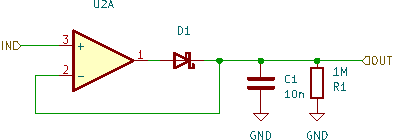
\includegraphics{img/peak_detector.pdf}
	\includesvg{img/peak_detector.svg}
	\caption{Przykładowy schemat połówkowego detektora szczytowego}
	\label{fig:peak-detector-schematic}
\end{figure}

\subsection{Element sprzęgający}
Wymagany jest układ umożliwiający tłumienie sygnału zmiennego względem sygnału sterującego:

\begin{equation}
	V_{wyj} \propto \frac{V_{wej}}{V_{ster}}
	\label{eq:coupling_1}
\end{equation}

Fizyczna implementacja takiego układu okazuje się być niebanalna.
Możliwy jest układ realizujący operacje mnożenia wartości sygnałów. 
Jego realizacja jednak jest wysoce złożona i wymaga relatywnie dużo części, 
ponieważ w jego skład wchodzą układy wyznaczające logarytm naturalny obu wartości, dodające te wartości do siebie,
a na koniec wyznaczające funkcje wykładniczą $e^x$ tej sumy.

Alternatywna metoda wykorzystuje element zmieniający swój opór elektryczny względem jakiegoś innego czynnika.
Przykładem historycznej realizacji takiego układu jest zastosowanie niewielkiej łapmy żarowej,
której opór włókna jest wprost proporcjonalny do jego temperatury.

Istnieje jednak znacznie prostsze i wydajniejsze rozwiązanie.

Popularnym elementem o zmiennym oporze jest fotorezystor. W przeciwieństwie do innych elementów
światłoczułych, przy stałym natężeniu światła, zachowuje się on jak faktyczny rezystor,
tzn. prąd przepływający jest wprost proporcjonalny do napięcia i odwrotnie do jego oporu
$I \propto \frac{V}{R_{\phi}}$.

Tak więc, jeśli zamknie się fotorezystor w obudowie światłoszczelnej wraz z diodą LED,
uzyskamy układ o zmiennym oporze elektrycznym, kontrolowany przez prąd diody\footnote{Zakładam $\phi \propto I$}.

\begin{equation}
	R \propto \frac{1}{I_{Led}}
\end{equation}

Umożliwia to łatwą implementacje układu sprzężenia (Eq. \ref{eq:coupling_1}). 

Co prawda powyższy model ignoruje fakt,
iż tak na prawdę opór fotorezystora zależny jest wykładniczo od natężenia padającego światła
$R = \left(\frac{1}{\phi}\right)^A$. Nie stanowi jednak to dużego problemu ponieważ układ ten znajduje się w 
pętli sprzężenia zwrotnego.

\begin{equation}
	R \propto \frac{1}{(I_{Led})^A}
\end{equation}

\subsection{Źródło odniesienia}
W tym momęcie potrzebne jest jedynie stabilne oraz dostrajalne źródło napięcia odniesienia.
Do tego celu z zupełności wystarczy układ LM4041 wraz z precyzyjnym potencjometrem.

\section{Implementacja}
\label{sec:impl}
Czas przejść do opisu kodu źródłowego.
W pliku \verb|sine_tab.cpp| znajduje się definicja tabeli funkcji sinus. Składa się ona z \verb|1024| próbek, a wartość \verb|i|-tej próbki 
zdefiniowana jest w następujący sposób:

\begin{equation}
	f(i) = (2^N - 1) + \left\lfloor (2^N - 1) \times \sin \left(\frac{2 \pi \times i}{N_{smpl}}\right)\right\rceil
\end{equation}
\begin{equation}
	f(i) = 127 + \left\lfloor 127 \times  \sin \left(\frac{2 \pi \times i}{1024}\right)\right\rceil
\end{equation}

Każda próbka jest 8-bitową liczbą całkowitą z zakresu $\in \{0 \dots 254\}$, jednocześnie tabela przedstawia cały jeden okres funkcji sinus,
poza wartością $\sin (2 \pi)$. Następną próbkę stanowi wartość $\sin (0)$. Dzięki temu reprodukowany sygnał nie zawiera przeskoku co cały okres.

Zadaniem oprogramowania mikrokontrolera pozostaje wczytanie kolejnych wartości z pamięci,
a następnie ustawienie pinów na odpowiedni stan. Wykorzystując 8-bitową naturę architektury AVR
możliwe jest ustawienie stanu całego rejestru (tj. grupy 8 pinów) poprzez pojedynczy zapis do 
obszaru peryferialnego pamięci (Linia \ref{code:set_pin_reg})

W tym miejscu napotykamy jednak pewien problem, synteza powyższego sygnału wymaga produkcji ponad miliona próbek na sekundę,
tym czasem zastosowany mikroprocesor jest przystosowany do pracy przy częstotliwości nie przekraczających \qty{24}{\MHz}.
Przy zastosowanym generatorze kwarcowym o częstotliwości pracy \qty{12,288}{\MHz} oznacza to, że mamy dokładnie \textbf{12} cykli maszynowych
na wygenerowanie następnej próbki, co więcej aby zachować precyzje częstotliwości musimy wykorzystać wszystkie 12 cykli za każdym razem.
Stąd też decyzja o implementacji całego algorytmu bezpośrednio w niskopoziomowym assemblerze.
Pozwala to na dokładną kontrolę nad czasem wykonania całego cyklu, a jednocześnie umożliwia szereg optymalizacji
będących poza zasięgiem kompilatora.

Kolejne bajty pobierane są przez instrukcje ld (Linia \ref{code:load_and_inc}), która jednocześnie
inkrementuje wskaźnik tworzony przez parę rejestrów \verb|r30| i \verb|r31|.

Problemem pozostaje jedynie wydajne zawijanie wskaźnika po dotarciu do 1024-tej wartości.
Ponownie wykorzystując 8-bitową nature układów AVR, możliwe jest bardzo wydajne rozwiązanie tego problemu.

Jednym z atrybutów udostępnianych przez kompilator GCC jest\\
\verb| __attribute__((aligned (1024)))|, który pozwala na wymuszenie
wyrównania pozycji pierwszego bajtu danej zmiennej do wielokrotności liczby podanej jako argument.
Oznacza to iż pozycja tablicy przyjmuje postać $A \times 1024$.

Tak więc, niższy bajt 16-bitowego wskaźnika będzie ulegał stałym zmianą na całej swojej długości,
natomiast w bajcie wyższym, dzięki wyrównaniu tabeli, zmieniać się będą jedynie dwa najniższe bity (Rys. \ref{fig:bits_ex}).

\begin{figure}[h]
	\centering
	\hfill

	\begin{bytefield}[bitwidth=7mm,endianness=big]{16}
		\bitheader{0-15} \\
		\bitbox{8}{r31} & \bitbox{8}{r30}\\
		\bitbox{6}{ \tt SINE\_TAB $\gg$ 10 } & \bitbox{10}{ Licznik }\\
	\end{bytefield}
	\caption{Schemat rozkładu bitów we wskaźniku}
	\label{fig:bits_ex}
\end{figure}

Tak więc jedyne co tak na prawdę musimy robić to nie pozwolić na zmianę stanu 6 najwyższych bitów wskaźnika.
Możemy to osiągnąć używając sprytej sztuczki, zajmującej łącznie 2 cykle zegarowe (Linia \ref{code:overflow_pointer}).

\begin{equation}
	r31' = \left( \left( r31 \lor 11_{bin} \right) \land r20 \right)
\end{equation}

Po pierwsze zerujemy sześć najwyższych bitów górnego rejestru instrukcją \verb|ANDI| - (And with Immidiate) z liczbą $3_{dec}$.
Następnie instrukcja \verb|OR| przywraca poprawny stan wyższych bitów, 
które na początku działania programu zostały zapisane w rejestrze 20 (Linijka \ref{code:set_r20_bp}).

\subsection{Dithering}
Techniką mogącą poprawić charakterystykę szumową sygnału jest tzw. Dihering. polegającą na uprzypadkowieniu najniższych bitów próbek.
Pozwala to na gładszy rozkład energii składowych wynikających z kwantyfikacji sygnału (Rys. \ref{fig:sine-stepped})
Korzyści jej stosowania nie zostały jeszcze ustalone na tym etapie projektu, jednak możliwa okazała się jej implementacja,
pomimo wysoce ograniczonych zasobów obliczeniowych.

W celu generowania przypadkowych bitów zaimplementowany został prosty generator LCG (Linia \ref{code:dither})

\begin{equation}
	r0'=3 \times r0 \mod 256
\end{equation}

Do tego celu wykorzystane zostały właściwości instrukcji \verb |MUL| mnożącej wartość dwóch rejestrów 8-bitowych,
a otrzymując 16-bitowy wynik zawarty w parze rejestrów \verb|r1, r0|.

Teraz jako wynik przypadkowej operacji zostaje wybrany 9-ty bit wyniku operacji $r0 \times 3$.
Zawarty jest w rejestrze \verb|r1|. Następnie XOR-owany jest z wartością następnej próbki zawartej w \verb|r2|

\begin{equation}
	r2' = r2 \oplus \left( \left( (r0 \times 3) \gg 8 \right) \land 1 \right)
\end{equation}


\subsection{Kod źródłowy}

\inputminted[linenos=true,escapeinside=@@,fontfamily=phv]{asm}{../src/main.S}

\newpage
\printbibliography %Prints bibliography

\newpage

\begin{figure}
	\centering
	
\includegraphics[width=0.75\textwidth]{img/kot_enter.jpg}
	\caption{Kot autora wspomagający proces twórczy}
\end{figure}

\end{document}